\documentclass[12pt]{article}

% Packages 
\usepackage{amsmath}
\usepackage{datetime}
\usepackage{graphicx}
\usepackage{listings}
\usepackage{gensymb}

\graphicspath{{./images/}}

\newdate{date}{11}{04}{2022}
\title{
    Assignment 22

    \large{
        ME EN 6240 Advanced Mechatronics
    }  
}
    
\author{
        Ryan Dalby
}
\date{\displaydate{date}}

\setlength\parindent{0pt}

\begin{document}
\maketitle

\section*{Exercise 2}

The following plots are generated by \verb|sound_test.m| which filters the desired tones using an FIR filter.
\begin{center}
    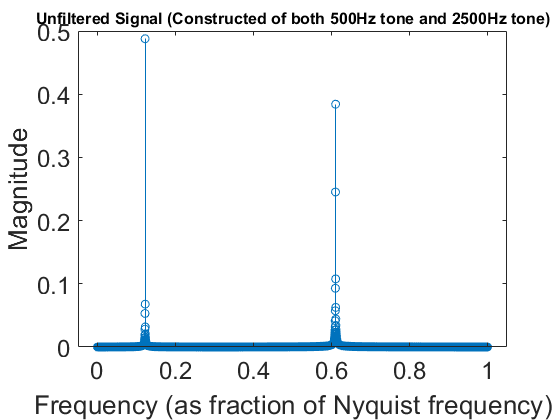
\includegraphics[width=4.8in]{unfiltered.png}

    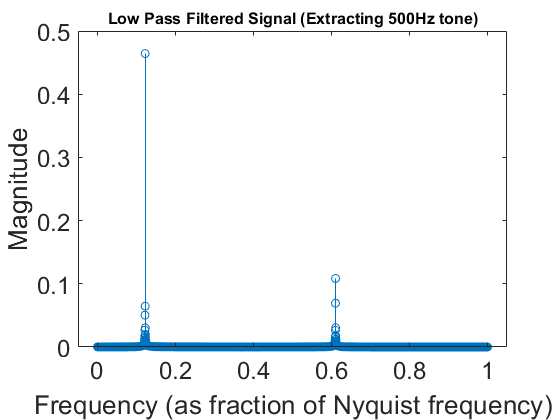
\includegraphics[width=4.8in]{lowpass_fir.png}

    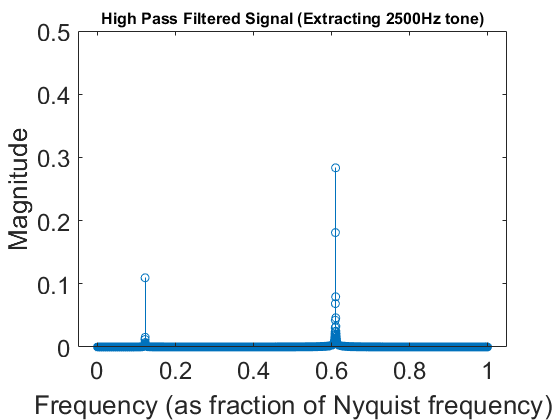
\includegraphics[width=4.8in]{highpass_fir.png}
\end{center}

\section*{Exercise 3}
See \verb|main.c| and \verb|readFIRValues.m| for top level filtering and communication code.

See \verb|FIR.c| and \verb|FIR.h| for FIR filtering library.

See \verb|getFIRCoeff.m| for how filtering coefficients were calculated.

These are the produced output plots (Note because there was no noise and the filter window was not big enough it is hard to observe the effect of the filter other than the shifting of the filtered signal):

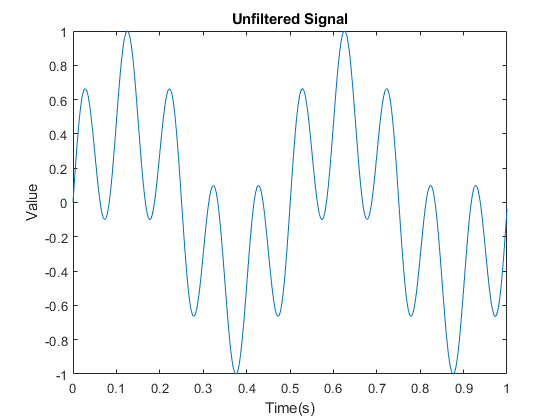
\includegraphics[width=5.1in]{3_u.png}

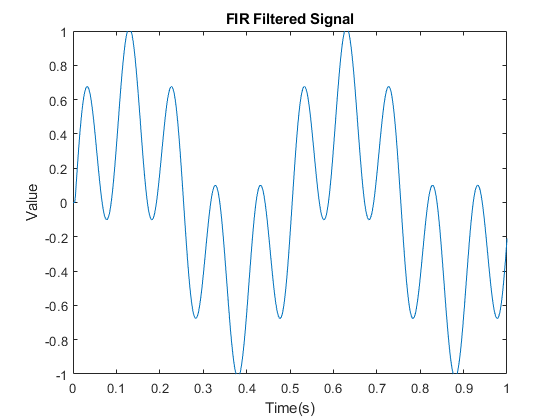
\includegraphics[width=5.1in]{3_f.png}

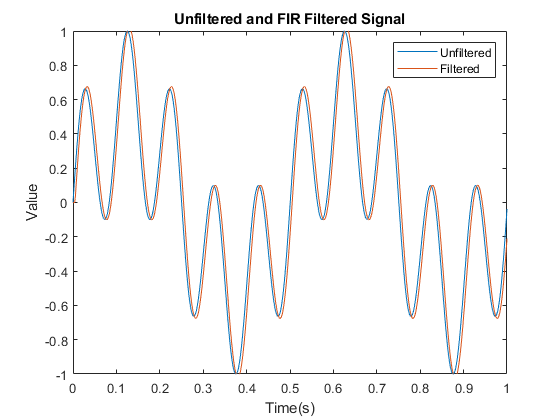
\includegraphics[width=5.1in]{3_fu.png}

\end{document}
